\documentclass{article}
\usepackage[utf8]{inputenc}
\usepackage{graphicx}
\usepackage{fancyhdr}
\usepackage{verbatim}
\usepackage[danish]{babel}
\pagestyle{fancyplain}
\author{Mikkel Kragh Mathiesen, Jannik Gram, Rune \& Rasmus Abrahams{\tt (son|en)}}
\title{}
\date{\today}
\lhead{Mikkel, Jannik, Rune \& Rasmus}
\rhead{\today}
\begin{document}

\maketitle

\section{Analyse af modellerings- og simuleringsprocesser}
\subsection*{(1.a)}
%Artiklen indeholder modellerne ``matematisk model'' og ``diskret model''; den indeholder processerne ``idealisering'' og ``diskretisering''.

%Den matematiske model består af ligninger.

%Artiklen præsenterer problemstillinger fra den virkelige verden omhandlende udfordringen med at afgøre hvordan de forskellige led på en robot eller et menneske skal bevæge sig for at opnå forskellige mål. Dette hører ind under boksen ``Real World''. Med dette i mente opstilles der en model under en proces, der retteligt kan betegnes som idealisering. Den resulterende model er matematisk af karakter og hører ind under boksen af samme navn. Til sidst ligger den matematiske model grund til udformningen af en algoritme, der hører ind under boksen ``diskret model''. Dette udgør processen ``diskretisering''.

%Artiklen verificerer ikke den diskrete model. Der er flere måder på hvilke dette kunne gøres. En mulig måde er formel verifikation af algoritmen ved brug af for eksempel Hoare-logik, men det praktiske aspekt af dette kan muligvis være for omfattende. En anden mulighed er et udføre dækkende afprøvninger.

%verification
%simulation
%results
%validation

\begin{itemize}
	\item
\begin{itemize}
	\item Boks: "Virkelige" verden \\
	Artiklen præsenterer problemstillinger fra den virkelige verden omhandlende udfordringen med at afgøre hvordan de forskellige led på en robot eller et menneske skal bevæge sig for at opnå forskellige mål.
	\item Pil: Idealisering \\
	I idealiseringsdelen handler det om at forsimple dele af den virkelige verden til håndgribelige modeller som kan beskrives matematisk. I artiklen idealiseres den menneskelige krop til stangmodellen, hvor kroppen omdannes til et simpelt skelet bestående af stænger og led.
	\item Boks: Matematisk model \\
	Den matematiske model handler om at opstille formler der kan beskrive hvordan det forsimplede menneske hænger sammen.
	\item Pil: Discretisering \\
	Den matematiske model gøres diskret. Gradienten $\rightarrow$ gættemodel% TODO?????
	\item Boks: Diskret model \\
	Den diskrete model går ud på at formlerne fra før tages i brug hvor man justerer variablene tilstrækkeligt indtil man får et passende resultat. % TODO Skriv noget om gradient?
	\item Pil: Simulering \\
	Artiklen simulerer ikke modellen. % NÅÅH TODO
	\item Boks: Resultater \\
	NEJ % TODO
	\item Pil: Validering \\
	NEJ % TODO
	\item Pil: Verificering \\
	Artiklen verificerer ikke den diskrete model.
\end{itemize}

\item
\begin{itemize}
	\item Pil: Simulering \\
	Den diskrete model kunne bruges til at laves konkrete eksempler. Som for eksempel at få modellen til at række ud efter en kop kaffe.
	\item Pil: Validering \\
	Ud fra simuleringen vil resultater for hvordan modellen ville tage en kop kaffe. Dennes bevægelser kan efterprøves af et menneske for at se om det er "lovlige" bevægelser.
	\item Pil: Verificering \\
	Der er flere måder på hvilke dette kunne gøres. En mulig måde er formel verifikation af algoritmen ved brug af for eksempel Hoare-logik, men det praktiske aspekt af dette kan muligvis være for omfattende. En anden mulighed er et udføre dækkende afprøvninger.
\end{itemize}
\end{itemize}

\subsection*{(1.b)}
% TODO

\section{Boldsimulator}

\begin{figure}
	\begin{verbatim}
		function [x, y, vx, vy] = ball_step(x, y, vx, vy, dt, m, g)
		    x = x + dt * vx
		    y = y + dt * vy
		    vy = vy - dt / (m * g)
		end
	\end{verbatim}
	\caption{ball\_step.m}
	\label{ballsinmyass}
\end{figure}

\subsection*{(2.a)}
På figur \ref{ballsinmyass} ses ball\_step.m.

\subsection*{(2.b)}
\begin{figure}
	\begin{verbatim}
		function [X Y] = ball_simulate(x0, y0, vx0, vy0, dt, m, g)
			x  = x0;
			y  = y0;
			vx = vx0;
			vy = vy0;

			X  = [];
			Y  = [];

			while y>=0
			  [x y vx vy] = ball_step(x,y,vx,vy,dt,m,g);
			  X = [X x];
			  Y = [Y y];
			end
		end
	\end{verbatim}
	\caption{ball\_simulate.m}
	\label{ballsims}
\end{figure}

På figur \ref{ballsims} ses ball\_simulate.m.

\subsection*{(2.c)}

\subsubsection*{1.}

I denne model er der tre parametre, som kan ændres. Der er tid $\Delta T$, masse $m$ og tyngdekraft $g$. Nedenfor ses en række forsøg:
\begin{itemize}
	\item Tyngdekraften 0 bør lave en lineær bane for bolden.
	\item En høj tyngdekraft lim->uendelig skulle gerne lade vores bold ligge fast
	\item Bolde med forskellig masse skulle gerne bevæge sig samme distance.
	\item Hvis vi har en høj tidsforskel skulle vi gerne få en mindre præcis måling end med en lav tidsforskel
\end{itemize}

\subsubsection*{2.}
Med lav tyngdekraft ville vi bruge T/(g*m) og g havde vi sat til 0. Vi kunne derfor ikke gennemføre testen da vi ikke kan dividere med 0.
Ved meget høj tyngdekraft (vi har dog kun sat den til 9000) blev den aldrig færdig med udregningen hvilket må betyde at bolden ikke faldt til jorden. Dette må betyde at vores matematiske model er forkert. Dette havde vi allerede mistanke om da Newton's anden lov, som er opgivet sammen med opgaveformulering ikke er korrekt.
Vi har forsøgt at "kaste bolde" med forskellig masse og vi fik forskellige resultater hvilket også betyder at vores matematiske model er forkert.
Ved forsøget med høj og lav tidsforskel var det tydeligt at se den med høj tidsforskel havde betydeligt mindre antal punkter og kurven var derfor tilpasset og gav et mere upræcist billede.

Vi kan altså konkludere at vores model ikke er korrekt i dette tilfælde og vi er nødt til at få de rigtige formler for at kunne komme skridtet videre og kunne validere.

\section{Kantfinder}

\subsection*{(3.a)}

\begin{figure}
	\begin{verbatim}
		function r = sobel_fold(A, B)
		    r = 0;
		    for i=1:3
		        for j=1:3
		            r = r + A(i,j)*B(i,j);
		        end
		    end
		end
	\end{verbatim}
	\caption{Kildekode til sobel\_fold.m}
	\label{sobelfold}
\end{figure}

\begin{figure}
	\begin{verbatim}
		function J = edge_detector(I)

		[M, N] = size(I);
		J = zeros( size(I) );

		Ex = [-1 -2 -1; 0 0 0; 1 2 1];
		Ey = [-1 0 1; -2 0 2; -1 0 1];

		for i=2:M-1
		  for j=2:N-1

		    A = zeros(3);

		    A(1,1) = I(i-1,j-1);
		    A(1,2) = I(i-1,j  );
		    A(1,3) = I(i-1,j+1);

		    A(2,1) = I(i  ,j-1);
		    A(2,2) = I(i  ,j  );
		    A(2,3) = I(i  ,j+1);

		    A(3,1) = I(i+1,j-1);
		    A(3,2) = I(i+1,j  );
		    A(3,3) = I(i+1,j+1);

		    val1 = sobel_fold(A, Ex);
		    val2 = sobel_fold(A, Ey);
		    J(i,j) = sqrt( val1^2 + val2^2 );
		  end
		end

		end
	\end{verbatim}
	\caption{Kildekode til edge\_detector.m}
	\label{edgedetector}
\end{figure}

Sobeloperationen er implementeret i funktionen på figur~\ref{sobelfold} og bruges i {\tt edge\_detector} på figur~\ref{edgedetector}.

Bemærk at koden ikke tager højde for problemer i forbindelse med gitterets yderste pixels. Således har en kantpixel forholdsmæssigt op til tre færre naboer at sammenligne sig med. Konsekvenserne af dette kan for eksempel ses på figur~\ref{ke1} og figur~\ref{ke1r}, hvor de to sorte linier mod forventning ikke helt når billedrammen.

\subsection*{(3.b)}

\subsubsection*{Verifikation}

Den diskrete model behøver umiddelbart ikke verificeres, idet afstanden mellem denne og den matematiske model er meget lille og overgangen direkte --- matrixoperationerne lader sig uden videre implementere.

\subsubsection*{Validering}
Med henblik på valideringen udsættes kantfinderen for en række forhåbentlig dækkende afprøvninger. Først et basistilfælde for at se, om den overhovedet virker efter hensigten; denne afprøvning består af et meget simpelt billede med et par sorte streger på hvid baggrund [\ref{ke1}, \ref{ke1r}]. Herefter testes diverse særtilfælde ved billeder uden tydelige kanter [\ref{ke2}, \ref{ke2r}] og billeder med har færre end tre pixels i hver dimension [\ref{ke5}, \ref{ke5r}]. Til sidst afprøves en slags grænsetilfælde --- her meget store billeder [\ref{ke4}, \ref{ke4r}], som programmet også gerne skulle kunne håndtere.

	\begin{figure}
		\centering
		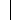
\includegraphics[width=3in]{test1.png}
		\caption{En streg --- bemærk at den rører billedrammen både i toppen og i bunden.}
		\label{ke1}
	\end{figure}
	\begin{figure}
		\centering
		
\includegraphics[width=4in]{test1_result.png}
		\caption{Kanterne af figur~\ref{ke1}.}
		\label{ke1r}
	\end{figure}
	\begin{figure}
		\centering
		
\includegraphics[width=3in]{test2.png}
		\caption{Flydende overgang (umiddelbart uden tydelige kanter).}
		\label{ke2}
	\end{figure}
	\begin{figure}
		\centering
		
\includegraphics[width=4in]{test2_result.png}
		\caption{Kanterne af figur~\ref{ke2}.}
		\label{ke2r}
	\end{figure}
	\begin{figure}
		\centering
		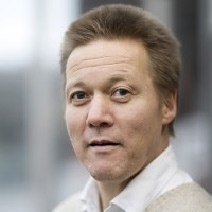
\includegraphics[width=3in]{test3.jpg}
		\caption{Jyrki Katajainen --- et ægte grænsetilfælde.}
		\label{ke3}
	\end{figure}
	\begin{figure}
		\centering
		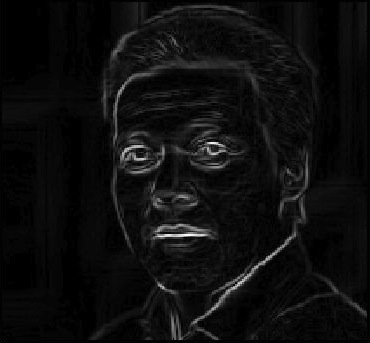
\includegraphics[width=4in]{test3_result.jpg}
		\caption{Kanterne af figur~\ref{ke3}.}
		\label{ke3r}
	\end{figure}
	\begin{figure}
		\centering
		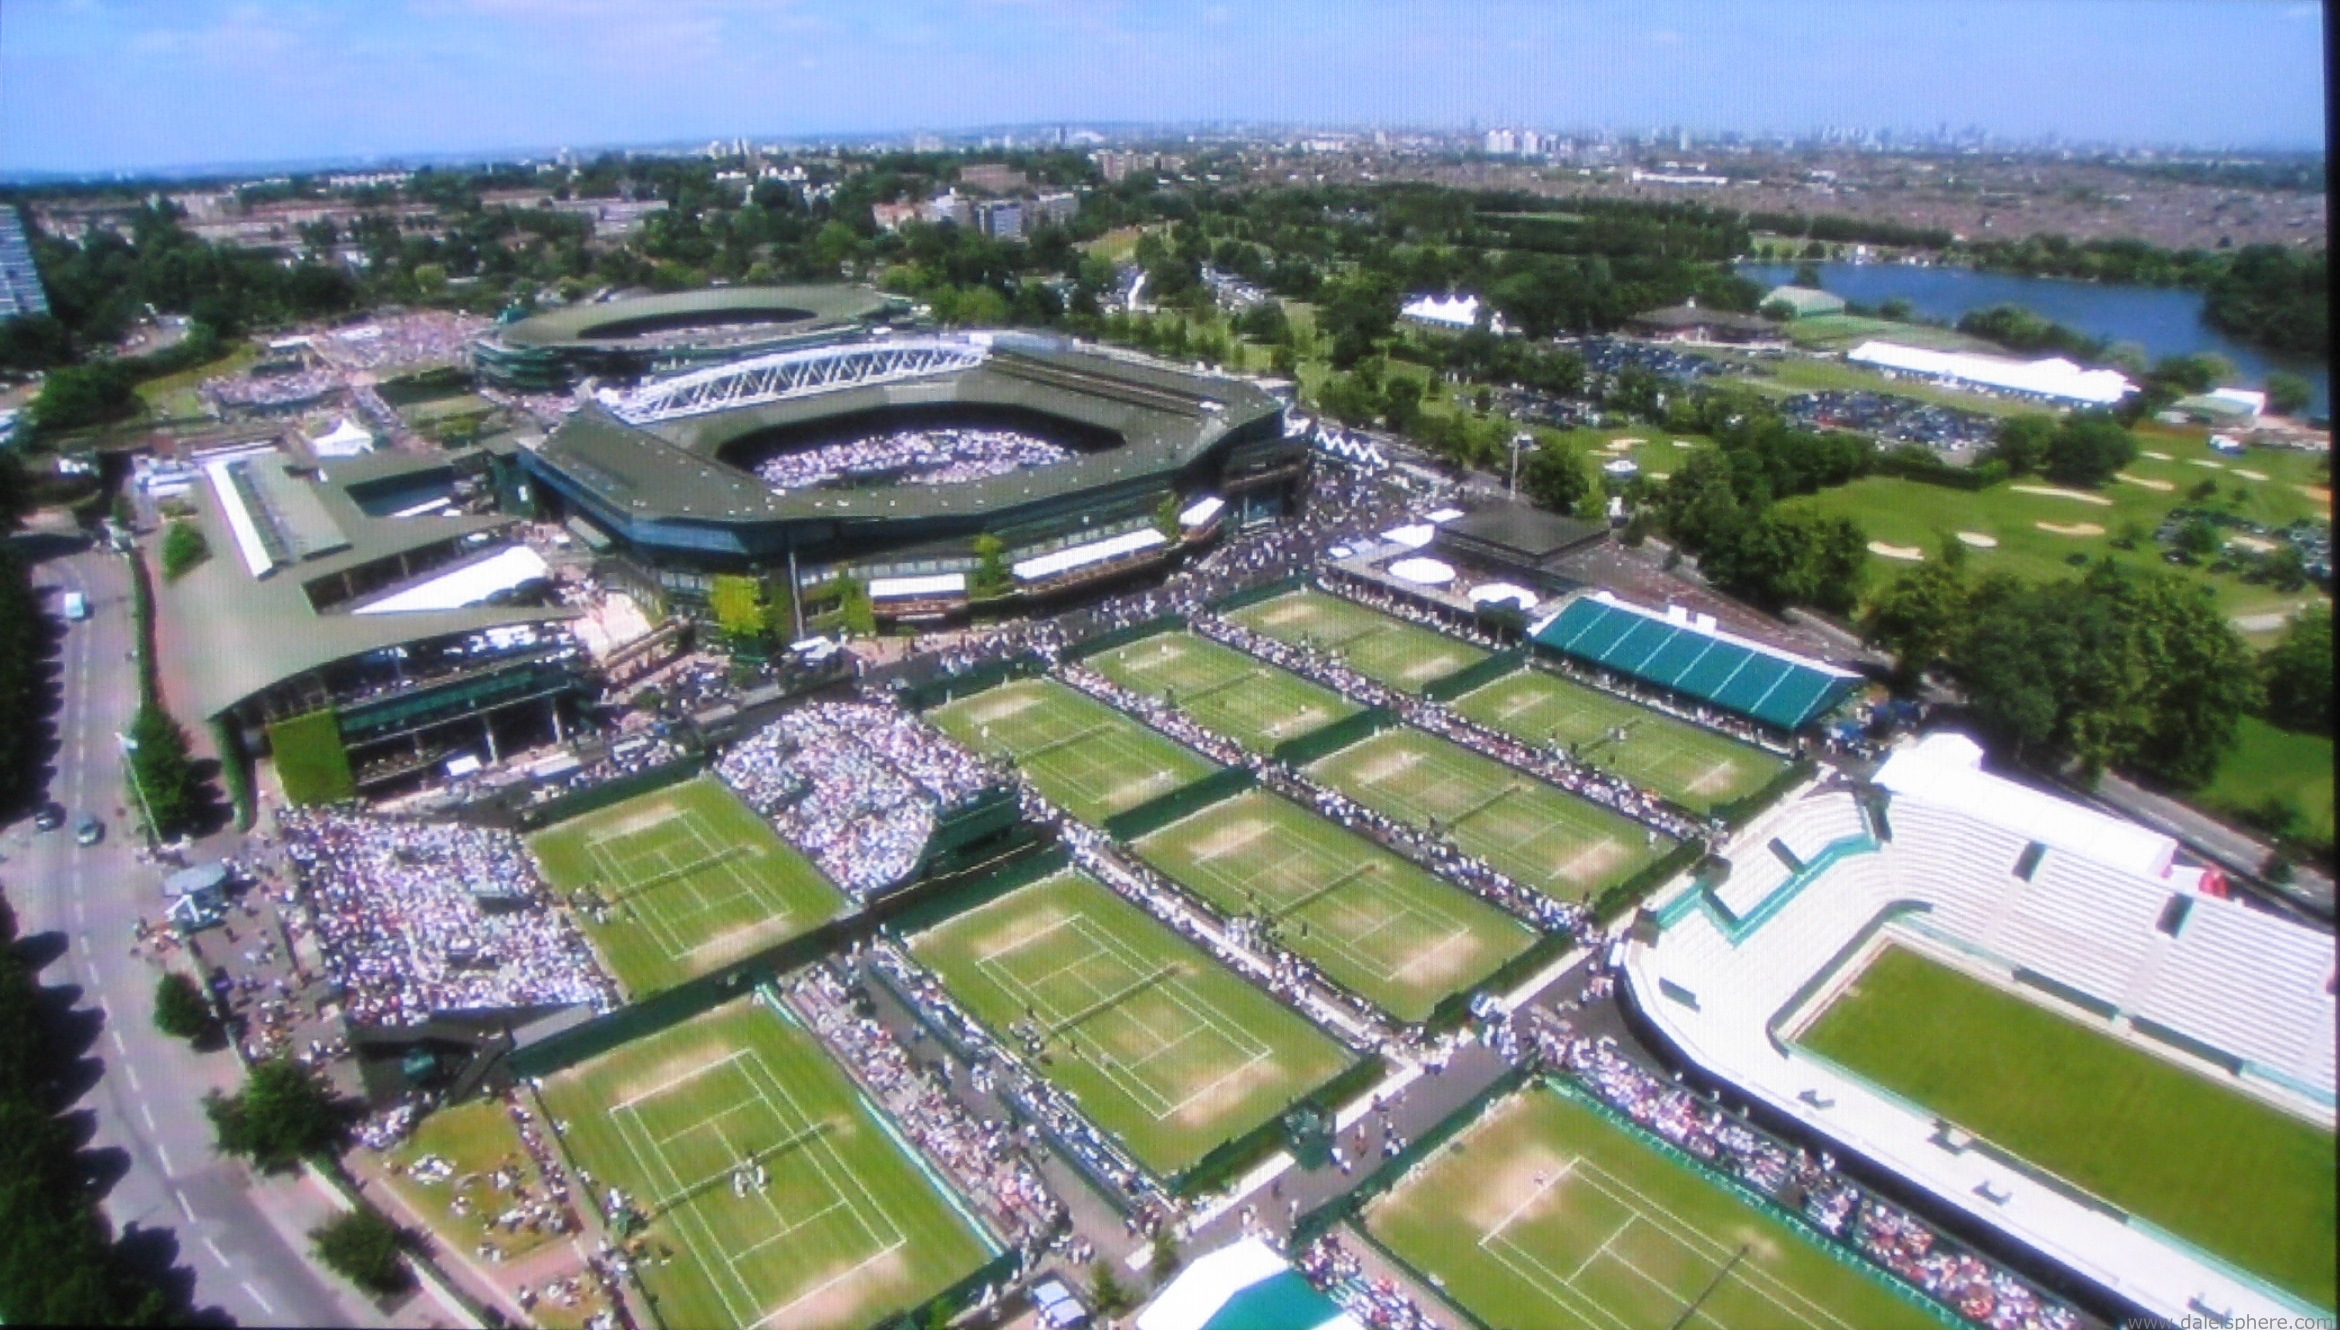
\includegraphics[width=4.5in]{test4.jpg}
		\caption{Et billede med høj opløsning.}
		\label{ke4}
	\end{figure}
	\begin{figure}
		\centering
		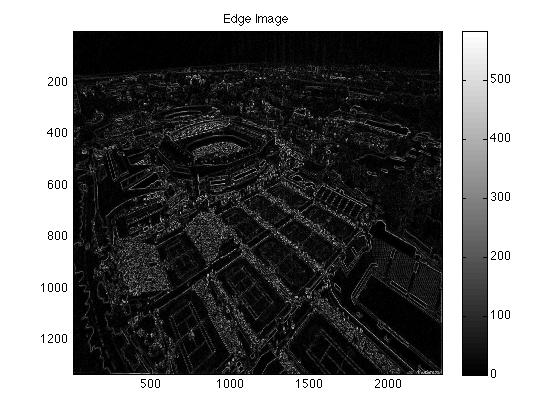
\includegraphics[width=6in]{test4_result.jpg}
		\caption{Kanterne af figur~\ref{ke4}.}
		\label{ke4r}
	\end{figure}
	\begin{figure}
		\centering
		
\includegraphics[width=3in]{test5.jpg}
		\caption{Et billede med få pixels.}
		\label{ke5}
	\end{figure}
	\begin{figure}
		\centering
		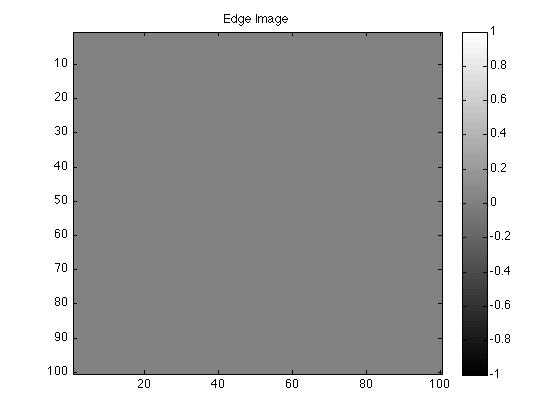
\includegraphics[width=4in]{test5_result.jpg}
		\caption{Kanterne af figur~\ref{ke5}.}
		\label{ke5r}
	\end{figure}

\end{document}
